%\documentclass[twoside]{pwrthesis}
\documentclass[twoside]{iisthesis}
% ---
\usepackage{polski}
\usepackage[utf8]{inputenc}
\usepackage{amsmath}
\usepackage{tocloft}
\usepackage{listings}
\usepackage{algorithm}
\usepackage{algorithmic}
\usepackage{subcaption}
\usepackage{mathtools}
\usepackage{graphicx}
\usepackage[colorinlistoftodos]{todonotes}
\usepackage{url}
\usepackage{pgfplots, pgfplotstable}
\selectlanguage{polish}
% Dodane przeze mnie d
\usepackage{fancyvrb} % dla srodowiska Verbatim
\usepackage{color}
\usepackage{lscape}
\hypersetup{
    colorlinks,
    linkcolor={black!50!black},
    citecolor={black!50!black},
    urlcolor={black!80!black}
}

\definecolor{gray}{rgb}{0.4,0.4,0.4}
\definecolor{darkblue}{rgb}{0.0,0.0,0.6}
\definecolor{cyan}{rgb}{0.0,0.6,0.6}

\lstset{
  basicstyle=\ttfamily,
  columns=fullflexible,
  showstringspaces=false,
  commentstyle=\color{gray}\upshape
}

\lstdefinelanguage{XML}
{
  morestring=[b]",
  morestring=[s]{>}{<},
  morecomment=[s]{<?}{?>},
  stringstyle=\color{black},
  identifierstyle=\color{darkblue},
  keywordstyle=\color{cyan},
  morekeywords={xmlns,version,type}% list your attributes here
}

\lstset{
  language=XML,
   literate={ć}{{\'c}}1
}
\renewcommand*{\lstlistingname}{Kod źródłowy}
% definicje kolorow
\definecolor{ciemnoSzary}{rgb}{0.15,0.15,0.15}
\definecolor{szary}{rgb}{0.5,0.5,0.5}
\definecolor{jasnoSzary}{rgb}{0.2,0.2,0.2}

% Konfiguracja verbatima
\fvset{
	frame=single,
	numbers=left,
	fontsize=\footnotesize,
	numbersep=12pt,
%	framerule=.5mm,
	rulecolor=\color{ciemnoSzary},
%	fillcolor=\color{jasnoSzary},
	framesep=4pt,
	stepnumber=1,
	numberblanklines=false,
	tabsize=2,
%	formatcom=\color{szary}
}
\newcommand{\listequationsname}{Spis wzorów}
\newcommand{\equationcaption}[1]{\begin{flushright}\emph{#1}\end{flushright}}
\newcommand{\rightcaption}[1]{\begin{flushright}\emph{#1}\end{flushright}}
\newlistof{myequations}{equ}{\listequationsname}
\newcommand{\myequations}[1]{%
\addcontentsline{equ}{myequations}{\protect\numberline{\theequation}#1}\par}

\newcommand{\listofmyalgorithmsname}{Spis algorytmów}
\newlistof{myalgorithm}{algo}{\listofmyalgorithmsname}
\newcommand{\myalgorithm}[1]{%
\addcontentsline{algo}{myalgorithm}{\protect\numberline{\thealgorithm}#1}\par}


\newcommand{\listofmyfiguresname}{Spis rysunków}
\newlistof{myfigure}{figu}{\listofmyfiguresname}
\newcommand{\myfigure}[1]{%
\addcontentsline{figu}{myfigure}{\protect\numberline{\thefigure}#1}\par}

\floatname{algorithm}{Algorytm}

\newtheorem{mydef}{Definicja}



\begin{document}


\newcommand{\resultChart}[7][140]{
\def\dataS{{#2}}
	\begin{figure}[H]
	
\centering

\begin{center}
\begin{tikzpicture}
 
\begin{axis}[
ybar,
bar width=20,
legend style={at={(0.5,-0.25)},
anchor=north,legend columns=-1},
ylabel={Wartość miary},
symbolic x coords={\dataS},
xtick=data,
height=  {#1},
width=0.8\textwidth,
ymin=0, ytick={0,0.5,1},
ymax=1.5,
nodes near coords,
nodes near coords align={vertical},
]
\addplot coordinates { (\dataS,{#3}) };
\addplot coordinates {(\dataS,{#4}) };
\addplot coordinates { (\dataS,{#5}) };
\legend{Recall,Precission,F1-Score}
\end{axis}
\end{tikzpicture}
\end{center}
\caption{{#6}}
\myfigure{{#6}}
\label{{#7}}
\end{figure}
}


\pgfkeys{/pgf/number format/use comma}
\pgfkeys{/pgf/number format/.cd, set thousands separator={}}%
\nocite{*}
\title{ TITLE }
\titleEN{ TITLE EN}
\shortTitle{SHORT TITLE}
\author{Katatzyna Biernat }
\advisor{dr inż. Bernadetta Maleszka}
\instituteLogo{logos/pwr}
\slowaKluczowe{KEYWORDS}

\date{\number\the\year}

% Wstawienie abstractu pracy
	%\input {abstract}

\abstractSH{SHORT ABSTRACT}

\abstractPL{
ABSTRACT PL
}
\abstractEN{
ABSTRACT EN
}

\maketitle
\textpages


\graphicspath{ {img/} }
\DeclareGraphicsExtensions{.pdf,.png,.jpg}

 \chapter{Cel pracy}
 \shortTitle{Cel pracy}
	Celem pracy jest zaproponowanie i zbudowanie hybrydowego algorytmu rekomendacji. Składowymi docelowego algorytmu są metody kolaboratywnego filtrowania oraz metody filtrowania z analizą treści.  
 
 \chapter{Wstęp}
 \shortTitle{Wstęp}
	 Wraz z rozwojem Internetu zmienił się sposób dostępu do informacji. Kiedyś to użytkownik musiał walczyć pozyskanie wiedzy; dzisiaj to informacje walczą u uwagę użytkowników. W świecie zalanym wiadomościami koniecznym wydaje się być zastosowanie filtra, który odsieje interesującą  i wartościową zawartość od tej niechcianej. Tak też z pomocą przychodzą zautomatyzowane mechanizmy rekomendacji.
	 
	 Jednakże sama idea rekomendacji nie jest niczym nowym. Co więcej, zjawisko to możemy zaobserwować w naturze -- na przykład wśród mrówek, które podążają wyznaczoną (rekomendowaną) ścieżką feromonową w poszukiwaniu pożywienia.
	 
	 Ludzie od niepamiętnych czasów posiłkowali się opiniami innych aby ułatwić sobie dokonanie wyboru, od najbliższego grona znajomych do ekspertów i autorytetów.
	 
	 Wraz z rozwojem nauk informatycznych problem rekomendacji stał się problemem interesującym badaczy. Za pierwszy system rekomendacji uznaje się \textit{Tapestry} stworzony w laboratoriach Xerox Palo Alto Research Center w 1992 roku. Motywacją było odfiltrowanie rosnącej liczby niechcianej poczty elektronicznej \cite{id:FromTapestryToSVD}.
	 
	 Wkrótce później idea ta została rozszerzona przez takich graczy jak Amazon, Google, Pandora, Netflix, Youtube, Yahoo etc. aż do formy, jaką znamy dzisiaj: systemu, który sugeruje użytkownikom produkty, filmy, muzykę, strony internetowe na podstawie ich aktywności w sieci \cite{id:EvolutionOfRecommenderSystems}. 
	 
	 Wielkie koncerny internetowe stale poprawiają jakość swoich algorytmów rekomendacji. Najlepszym przykładem jest tutaj Netflix, który w październiku 2006 zorganizował ogólnodostępny konkurs na najlepszy algorytm. Zadaniem uczestników było ulepszenie algorytmu Cinematch. Już po siedmiu dniach od ogłoszenia konkursu trzy zespoły zdołały przebić Cinematch o 1.06\% \cite{id:NetflixPrize}\cite{id:NetflixPrizeRankings}. 18 września 2009 Netflix ogłosił, że zespół BellKor's Pragmatic Chaos poprawił Cinematch o 10,06\% osiągając wynik $RMSE = 0.8567$. Tym samym wygrał nagrodę w wysokości \$1,000,000 i zakończył konkurs \cite{id:NetflixPrize2}\cite{id:NetflixPrizeRules}.
	 
	 Systemy rekomendacji ulepszane są nieustannie, o czym świadczy chociażby organizowana rokrocznie konferencja\textit{ ACM International Conference on Recommender Systems}. Tematyka ta poruszana jest także na konferencjach \textit{European Conference on Information Retrieval}, \textit{European Conference on Machine Learning and Principles and Practice of Knowledge Discovery in Databases} i wielu innych. Mimo dużego stopnia zaawansowania wciąż istnieje pole manewru do ulepszania algorytmów rekomendacji i co za tym idzie zwiększanie zadowolenia użytkowników, które z kolei prowadzi do osiągania korzyści biznesowych.
	 
 
 \chapter{Przegląd istniejących rozwiązań}
 \shortTitle{Przegląd istniejących rozwiązań}
	 Tradycyjnie wyróżniamy następujące techniki rekomendacji: \cite{id:IntroductionToRecommenderSystemsHandbook}
	 
	 \begin{itemize}
	 	\item \textbf{filtrowanie w oparciu o aktywność użytkownika} (eng. content-based), technika koncentrująca się na danych historycznych. Użytkownikowi rekomendowane są elementy, które podobne są do tych wybieranych przez niego w przeszłości;
	 	\item \textbf{filtrowanie kolaboratywne} (eng. collaborative filtering), technika polegająca na odnajdywaniu użytkowników o podobnych gustach i sugerowaniu lubianych przez nich elementów aktualnie aktywnemu użytkownikowi;
	 	\item \textbf{filtrowanie demograficzne} (eng. demographic), technika koncentrująca się na sugerowaniu aktywnemu użytkownikowi elementów popularnych pośród użytkowników z tej samej okolicy bądź w podobnym przedziale wiekowym;
	 	\item \textbf{filtrowanie z analizą domeny wiedzy} (eng. knowledge-based), technika dobierająca kolejne elementy na podstawie określonej domeny wiedzy na temat tego, jak dany element spełnia potrzeby i preferencje użytkownika;	
	 	\item \textbf{filtrowanie z analizą społecznościową} (eng. community-based), technika dobierająca rekomendacje dla użytkownika w zależności od preferencji innych użytkowników z jego sieci społecznościowej. W myśl zasady "powiedz mi kim są twoi przyjaciele a powiem ci kim jesteś";
	 	\item \textbf{hybrydowe systemy rekomendacji}, to kombinacja dowolnych powyższych technik.
	 \end{itemize}
	 
	 Każda z tych technik ma swoje wady i zalety w zależności od kontekstu, w którym ma być stosowana. 
	 
	 \section{Filtrowanie w oparciu o aktywność użytkownika}
	 
	 @TODO
	 
	 \subsection{Explicit/implicit feedback}
	 
	 Informacje na temat preferencji użytkownika mogą być zbierane na różne sposoby. Jeżeli użytkownik jawnie pozostawia informacje można mówić o bezpośredniej informacji zwrotnej (explicit feedback). Do takich informacji należą: ocena konkretnych elementów, tzw. łapka w górę lub w dół, komentarz itp. 
	 
	 Jednakże nawet jeżeli użytkownik nie jest skory do zostawiania tego typu śladów, to i tak można wiele na jego temat wywnioskować korzystając z informacji zwrotnych niejawnych (implicit feedback). System bierze wówczas pod uwagę aktywność użytkownika taką jak: historia zakupów, historia przeglądarki a nawet ruchy myszką. W przypadku serwisu z muzyką czy filmem cenną informacją będzie fakt, czy użytkownik wysłuchał lub obejrzał dany materiał do końca czy też wyłączył go po paru sekundach. \cite{id:ContentBasedRecommenderSystemsState}\cite{id:AdvancesInCollaborativeFiltering}
	 
	 \subsection{Najczęściej spotykane problemy}
	 Aby rekomendacja była skuteczna użytkownik powinien ocenić jak najwięcej elementów. Problematyczni są zatem użytkownicy, którzy dopiero co dołączyli do serwisu oraz tacy, którzy nie są aktywni i rzadko zostawiają po sobie ślad 	 \cite{id:MaleszkaMianowskaNguyenmethod}.
	 
	 \section{Filtrowanie kolaboratywne}
	 
	 Tradycyjnym i zarazem najprostszym podejściem do metody filtrowania kolaboratywnego jest rekomendowanie aktywnemu użytkownikowi elementów, które inni użytkownicy o podobnym guście uznali za atrakcyjne\cite{id:IntroductionToRecommenderSystemsHandbook}\cite{id:CollaborativeFilteringRecommenderSystems}. Użytkownicy o podobnym guście to osoby, które oceniły konkretne elementy podobnie jak aktywny użytkownik. 
	 
	 W przypadku filtrowania kolaboratywnego można wyróżnić dwa główne podejścia: oparte o regułę sąsiedztwa (ang. \textit{neighborhood methods}) oraz oparte o modele ukrytych czynników (ang. \textit{latent factor models})\cite{id:MatrixFactorizationTechniquesForRecommenderSystems}. 
	 
	 \begin{figure}[!ht] 
	 	\centering
	 	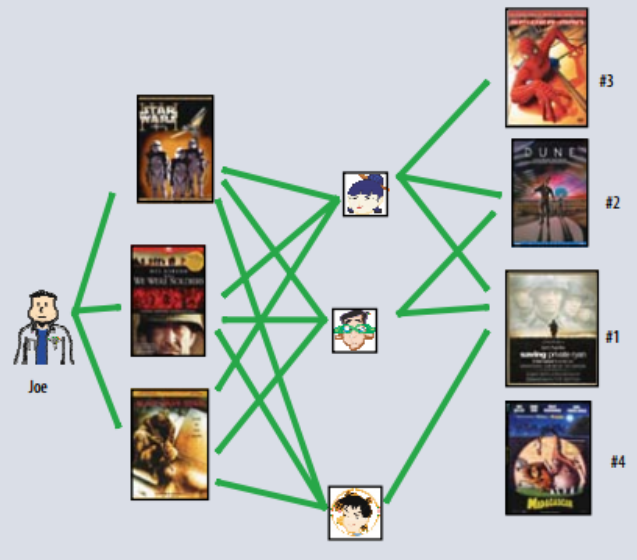
\includegraphics[width=0.7\textwidth]{cf}
	 	\caption{Filtrowanie kolaboratywne metodą sąsiedztwa zorientowanego na użytkownika\protect\cite{id:MatrixFactorizationTechniquesForRecommenderSystems}.}
	 	\label{fig:cf}
	 \end{figure}
	 
	 Rysunek \ref{fig:cf} pokazuje filtrowanie kolaboratywne oparte o regułę sąsiedztwa, zorientowane na użytkownika. Joe ocenił pozytywnie trzy filmy. System odnajduje innych użytkowników, którzy także ocenili te trzy filmy i dodatkowo kilka innych. Każdy z tych użytkowników pozytywnie ocenił film ,,Saving Private Ryan", zatem jest to pierwsza rekomendacja dla Joe. 
	 
	  \begin{figure}[!ht] 
	  	\centering
	  	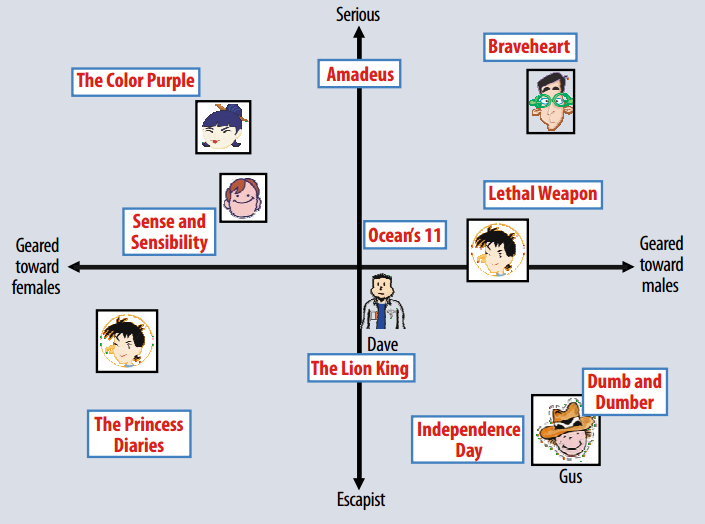
\includegraphics[width=0.7\textwidth]{cf2}
	  	\caption{Filtrowanie kolaboratywne z wykorzystaniem modeli ukrytych czynników\protect\cite{id:MatrixFactorizationTechniquesForRecommenderSystems}.}
	  	\label{fig:cf2}
	  \end{figure}
	 
	 Rysunek \ref{fig:cf2} pokazuje w sposób uproszczony podejście z wykorzystaniem ukrytych czynników. W układzie współrzędnym oznaczeni są użytkownicy wedle swoich preferencji oraz konkretnych cech (np. płeć) a także filmy, które stanowią odpowiedź na dany zestaw preferencji/cech \cite{id:MatrixFactorizationTechniquesForRecommenderSystems}. 
	 	 
	 \subsection{Najczęściej spotykane problemy}
	 
	 Jednym z problemów klasycznego podejścia do kolaboratywnego filtrowania jest brak uwzględnienia dynamiki zmian w gustach użytkowników. Ten sam użytkownik na przestrzeni kilku lat lub miesięcy może zupełnie inaczej ocenić ten sam film bądź piosenkę. Rozwiązaniem jest dodanie czynnika czasu podczas obliczania wag kolejnych ocen. \cite{id:NewRecommentationAlgoritmBasedOnSocialNetwork}\cite{id:NextSongRecommendationWithTemporalDynamics}\cite{id:MatrixFactorizationTechniquesForRecommenderSystems}.
	 
	 Innym problemem jest tzw. zimny start (eng. cold start). Polega on na tym, że użytkownicy nowi w systemie ocenili zbyt mało elementów, aby można było zbudować dla nich dobre rekomendacje\cite{id:zhang2015hybrid}\cite{id:RubensRecSysHB2010}.
	 
	 Powszechnym zjawiskiem jest tzw. efekt długiego ogona. Rysunek \ref{fig:longtail} przedstawia jak rozkłada się procentowa ilość ocen danych elementów w zależności od ich popularności. Jeżeli algorytm rekomendacji nie wspiera mniej popularnych elementów, to istnieje ryzyko, że użytkownicy nie otrzymają możliwości eksplorowania nowych, niszowych materiałów\cite{id:RubensRecSysHB2010}\cite{id:celma2010music}.
	 
  \begin{figure}[!ht] 
 	  	\centering
 	  	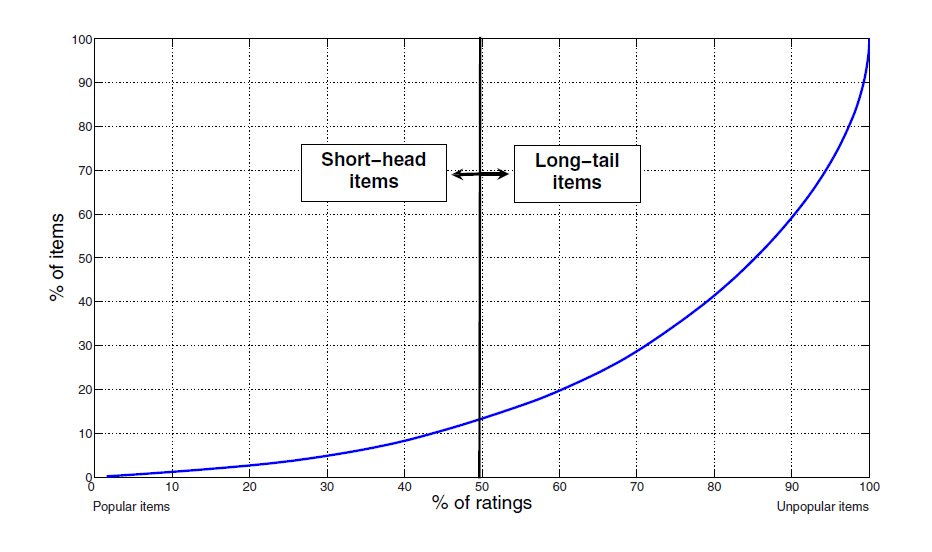
\includegraphics[width=0.7\textwidth]{longtail}
 	  	\caption{Problem długiego ogona: 50\% ocen dotyczy 10-12\% najpopularniejszych elementów w systemie\protect\cite{id:RubensRecSysHB2010}.}
 	  	\label{fig:longtail}
  \end{figure}
	 
	 Systemy rekomendacji wykorzystujące filtrowanie kolaboratywne nie są skalowalne. Złożoność rośnie proporcjonalnie do ilości użytkowników i elementów. Wielkie koncerny internetowe takie jak Twitter wykorzystają klastry i maszyny z bardzo dużą ilością pamięci aby zachować płynność działania serwisu \cite{id:gupta2013wtf}.
	 
	 \section{Popularne serwisy wykorzystujące algorytmy rekomendacji}
	 
	 @TODO - dokończyć 
	 
	 Algorytmy rekomendacji napotkać można praktycznie w większości dużych serwisów internetowych.
	 
		 \subsection{Rekomendacja muzyki}
	 
		 \begin{itemize}
		 	\item \textbf{YouTube} -- serwis powstały w 2005 roku, pozwalający na bezpłatne umieszczanie, odtwarzanie, ocenianie i komentowanie filmów. Od 2006 roku przejęty przez Google \cite{website:googleTakesYT}. YouTube buduje profil użytkownika w oparciu o jego aktywność w serwisie. Brane pod uwagę są polubienia (łapka w górę), subskrypcje, udostępnianie a także informacje czy użytkownik obejrzał film do końca czy tylko pewien jego procent \cite{id:TheYouTubeVideoRecommendationSystem}. Techniki rekomendacji stosowane przez serwis to przede wszystkim asocjacyjna eksploracja danych i licznik wspólnych odwiedzin danego wideo w czasie trwania pojedynczej sesji \cite{id:TheYouTubeVideoRecommendationSystem}. 
		 	\item \textbf{LastFM } -- internetowa radiostacja oferująca rozbudowany mechanizm rekomendacji piosenek ''Audioscrobbler''.   
		 	\item \textbf{Pandora}	
		 \end{itemize}
	 
		 \subsection{Rekomendacja filmów}
		 \begin{itemize}
			 \item \textbf{Netflix}
			 \item \textbf{Filmweb}
			 \item \textbf{IMDB}
		 \end{itemize}
		 
		 \subsection{Platformy typu e-commerce}
	
		\begin{itemize}
			 \item \textbf{Allegro}
			 \item \textbf{Amazon}
		 \end{itemize}	 
	 
		 \subsection{Inne serwisy}
		 
		 \begin{itemize}		 	
		 	\item \textbf{Google search}
		 \end{itemize}
 
 
 \chapter{Model systemu}
 \shortTitle{Model systemu}
 
 \chapter{Algorytmy}
 \shortTitle{Algorytmy}
	 \section{Filtrowanie kolaboratywne}
		 \subsection{Matrix Factorization}
		 \subsection{Biased Matrix Factorization}
		 \subsection{SVD++}
	 \section{Filtrowanie z analizą zawartości}
		 \subsection{Konstrukcja sieci neuronowej}
		 \subsection{Uczenie sieci neuronowej}
	 \section{Algorytymy hybrydowe}
	 \section{Analiza złożoności i poprawności}
 
\chapter{Ocena eksperymentalna}
\shortTitle{Ocena eksperymentalna}
	\section{Opis metody badawczej}
	\section{Środowisko symulacyjne}
	\section{Metodologia}
	\section{Przeprowadzone eksperymenty}
	
\chapter{Wnioski}
\shortTitle{Wnioski}

\chapter{CHAPTER 1}
\section{SECTION}

\def\alghoritm1{Alghoritm 1}
\begin{algorithm}
\caption{\alghoritm1}
\myalgorithm{\alghoritm1}
\label{aq:algStat}
\begin{algorithmic}
\STATE $T \leftarrow \text{text under analysis}$
\FOR{each word $w \in T$}
    \STATE $S_{w}\leftarrow FIND\_SENTIMENT(w) $
    \IF {$S_{w}=POSITIVE$}
        \STATE $Sentiment[POSITIVE]++$
    \ELSIF{$S_{w}=NEGATIVE$}
        \STATE $Sentiment[NEGATIVE]++$
    \ELSE 
        \STATE $Sentiment[NEUTRAL]++$
    \ENDIF
\ENDFOR
%\STATE $x\in\{POSITIVE,NEGATIVE,NEUTRAL\}$
\RETURN $\arg\max_x Sentiment[x]$
\end{algorithmic}
\end{algorithm}


\def\schema1{Schema 1}
\begin{figure}[ht]
\caption{\schema1}
\myfigure{\schema1}
\label{fig:kdb}
\begin{center}
    <GRAPHIC>
\end{center}
\end{figure}

\section{Section 2}

\subsection{Subsection 1}

\subsubsection{Subsubsection 1}

\begin{mydef}
\textbf{Definicja} - pierwsza
\end{mydef}



 \clearpage
\appendix
\chapter{Appendix 1}


\clearpage
\pagestyle{plain}
\listofmyfigure
\listofmyequations
\listofmyalgorithm
\clearpage

%\bibliographystyle{apalike}%Used BibTeX style is unsrt

\bibliographystyle{iisthesis}
\bibliography{bibliography}

\end{document}

